% Beispiel eines Kapitels für die Latex-Vorlage am ETI.
%--------------------------------------------------------------------
%
%   Version: 3.25        (Koma-Skript, documentclass{scrbook})
%   Datum: 01.06.2018
%   Autor: Johannes Bier
%
%--------------------------------------------------------------------

\chapter{Setup}
\section{Installation}
In diesem Kapitel wird beschrieben, welche Programme benutzt werden und wie diese Konfiguriert werden müssen, um diese Vorlage in vollem Umfang zu nutzen.

\subsection{MiKTeX}
Es wird die neuste Version von MiKTeX benötigt. Diese kann von \url{https://miktex.org/} für das jeweilige Betriebssystem heruntergeladen werden. 

\subsection{Perl}
Falls diese Vorlage auf einem Windows System benutzt wird, ist zusätzlich Perl notwendig. Diese Vorlage wurde mit Strawberryperl getestet und erstellt (\url{http://strawberryperl.com/}). Strawberryperl kann auch genutzt werden, wenn keine Admin-Rechte auf dem jeweiligen Computer vorhanden sind.
Auf Linux Systemen kann Perl falls notwendig mit \verb|sudo apt-get install perl| nachinstalliert werden.

\subsection{TeXstudio}\label{sec:texstudioconfig}
Es wird die neuste Version von TeXstudio benötigt. \url{https://www.texstudio.org/}

\textbf{Achtung:} MiKTeX sollte vor TeXstudio installiert werden!

Damit TeXstudio das Abkürzungs- sowie das Symbolverzeichnis automatisch mit erstellt, muss TeXstudio noch etwas konfiguriert werden. Die einzelnen Schritte zur genauen Konfiguration sind in \autoref{fig:texstudio_config} zu sehen.
 
 \begin{figure*}[p]
 	\centering
 	\begin{subfigure}[b]{0.475\textwidth}
 		\centering
 		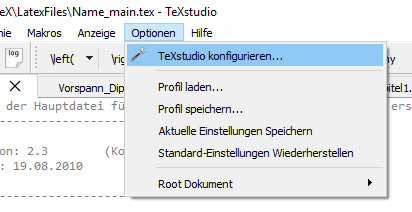
\includegraphics[width=\textwidth]{Nomencl_TexStudio_1.png}
 		\caption[Reiter $\rightarrow$ Optionen $\rightarrow$ TeXStudio konfigurieren...]{{\small Optionen $\rightarrow$ TeXStudio konfigurieren...}}    
 		\label{abb:texstudio_conf_1}
 	\end{subfigure}
 	\hfill
 	\begin{subfigure}[b]{0.475\textwidth}  
 		\centering 
 		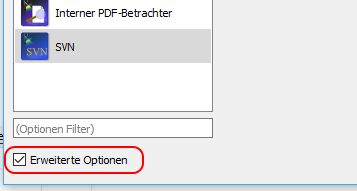
\includegraphics[width=\textwidth]{Nomencl_TexStudio_2.png}
 		\caption[Unten Links $\rightarrow$ Erweiterte Optionen]{{\small Unten Links $\rightarrow$ Erweiterte Optionen}}    
 		\label{abb:texstudio_conf_2}
 	\end{subfigure}
 	\vskip\baselineskip
 	\begin{subfigure}[b]{0.95\textwidth}   
 		\centering 
 		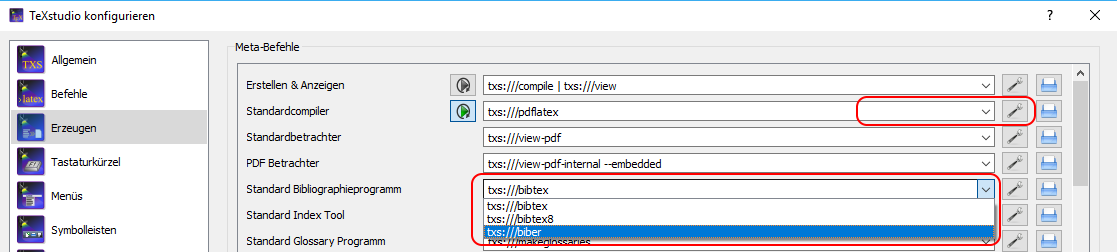
\includegraphics[width=\textwidth]{Nomencl_TexStudio_3.png}
 		\caption[Erzeugen $\rightarrow$ Standard Bibliographieprogramm $\rightarrow$ biber und  Erzeugen $\rightarrow$ Standardcompiler $\rightarrow$ Konfigurieren]{{\small Erzeugen $\rightarrow$ Standard Bibliographieprogramm $\rightarrow$ biber\\  Erzeugen $\rightarrow$ Standardcompiler $\rightarrow$ Konfigurieren}}    
 		\label{abb:texstudio_conf_3}
 	\end{subfigure}
 	\vskip\baselineskip
 	\begin{subfigure}[b]{0.95\textwidth}   
 		\centering 
 		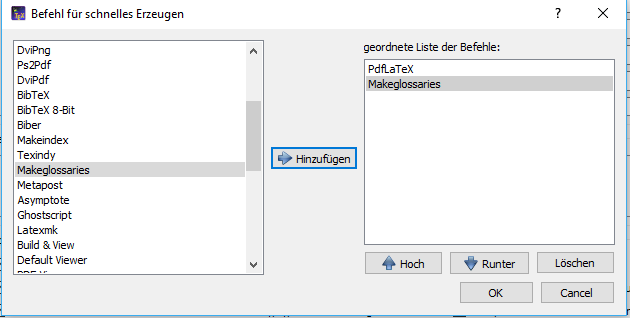
\includegraphics[width=\textwidth]{Nomencl_TexStudio_4.png}
 		\caption[Makeglossaries hinzufügen]{{\small Makeglossaries hinzufügen}}    
 		\label{abb:texstudio_conf_4}
 	\end{subfigure}
 	\caption[TeXstudio konfigurieren]{\small TeXstudio konfigurieren} 
 	\label{fig:texstudio_config}
 \end{figure*}
 
\chapter{Latex Grundlagen mit dieser Vorlage}
Das Dokument wird durch die Hauptdatei \verb|Name_main.tex| erzeugt. Zum bearbeiten sollte diese Datei immer als erstes geöffnet werden. TeXstudio erkennt dann automatisch welche Dateien zusätzlich eingebunden werden und zeigt diese auf der linken Seite an. Das Erstellen der Vorlage lässt sich von jeder Hierarchiestufe auslösen. 

In der Hauptdatei folgt der eigentliche Inhalt des Dokuments. Zunächst wird die Titelseite erstellt, die fast unverändert übernommen werden kann. Es müssen lediglich einige Daten, wie Name, Betreuer, Titel, etc. Weiter unten in \verb|Titelseite_Name.tex| muss auch noch die Kurzfassung und die Danksagung verfasst werden. Es empfiehlt sich die einzelnen Kapitel der Arbeit zur besseren Übersichtlichkeit in separaten Dateien zu verfassen, die mit \verb|\include{}| oder \verb|\input{}| in das Dokument eingefügt werden. 

Dieses Beispielkapitel sollte aus der Arbeit entfernt werden. Sollten jedoch Fragen und Unklarheiten auftreten, soll dieses Kapitel als Beispiel dienen, wie die einzelnen Inhalte erstellt werden.

\section{Absätze und Zeilenumbrüche}
Zeilenumbrüche werden von \LaTeX{} automatisch erzeugt und sollten \textbf{nicht} mit einem Befehl, wie \verb|\\| erzeugt werden. Um einen Absatz zu erzeugen, wird einfach eine Leerzeile zwischen den Textblöcken gelassen.

Möchte man die Silbentrennung eines Wortes verändern bzw. korrigieren kann man die Trennstellen des Wortes so angeben: \verb|Trenn\-stel\-len|. Möchte man das kein Zeilenumbruch zwischen zwei Wörtern, einem Wort und deinem Formelzeichen oder einem Wort und einer Zahl, so setzt man anstelle eines Leerzeichens eine Tilde \verb|(~)|.

\section{Aufzählungen}
\subsection{Punktiert}
Punktierte Aufzählungen werden mit der \verb|itemize|-Umgebung erzeugt.
\begin{lstlisting}[style=latex]
\begin{itemize}
	\item Erster Punkt.
	\item Zweiter Punkt.
\end{itemize}
\end{lstlisting}
\begin{itemize}
	\item Erster Punkt.
	\item Zweiter Punkt.
\end{itemize}
\subsection{Nummeriert}
Nummerierte Aufzählungen werden mit der \verb|enumerate|-Umgebung erzeugt.
\begin{lstlisting}[style=latex]
\begin{enumerate}
	\item Erster Punkt.
	\item Zweiter Punkt.
\end{enumerate}
\end{lstlisting}
\begin{enumerate}
	\item Erster Punkt.
	\item Zweiter Punkt.
\end{enumerate}

\section{Referenzen im Dokument}
Referenzen können auf verschiedenste Objekte mit \verb|\label{präfix:name}| erzeugt und mit  \verb|\autoref{präfix:name}| referenziert werden. Dabei ist es sinnvoll die Labels mit einem sinnvollen Namen und einem Präfix, der angibt um was für eine Referenz es sich handelt, zu versehen. 

\verb|\autoref| fügt mithilfe das \verb|Babel|-Pakets automatisch den Typ der Referenzierung z.B. Abbildung oder Tabelle vor der dazugehörigen Nummer ein. Der \verb|\label|-Befehl muss bei Kapiteln immer hinter dem Kapitel stehen.
\begin{lstlisting}[style=latex]
\chapter{name}\label{sec:kapitelname}
\section{name}\label{sec:sectionname}
\end{lstlisting}
Wo bei Abbildungen, Tabellen, usw. der \verb|\label|-Befehl stehen muss, wird in dem jeweiligen Kapitel erläutert.

Der Präfix hilft lediglich dem Autor den Überblick über das Dokument zu behalten und spielt keine Rolle dabei, welcher Typ wirklich referenziert wird. Damit das ganze aber etwas einheitlich bleibt hat man sich auf einige standardisierte Präfixe geeinigt. Die Liste der Präfixe ist in \autoref{tab:refprefixlabel} zu sehen.

\begin{table}[h]
	\centering
	\caption{Tabelle gängiger Präfixe für Referenzen.}
	\label{tab:refprefixlabel}
	\begin{tabular}{@{}C{2cm}L{5.5cm}@{}}
		\rowcolor[HTML]{000000} 
		{\color[HTML]{FFFFFF} \textbf{Präfix}} & {\color[HTML]{FFFFFF} \textbf{Beschreibung}}\\
		
		\rowcolor[HTML]{FFFFFF} 
		\verb|sec| & Kapitel und Unterkapitel\\
		
		\rowcolor[HTML]{C0C0C0} 
		\verb|fig| & \\
		\rowcolor[HTML]{C0C0C0} 
		\verb|abb| & \multirow{-2}{*}{\cellcolor[HTML]{C0C0C0}{Abbildungen}} \\ 
		
		\rowcolor[HTML]{FFFFFF} 
		\verb|eq|  & Formeln und Gleichungen\\
		
		\rowcolor[HTML]{C0C0C0} 
		\verb|tab| & Tabellen\\
		
		\rowcolor[HTML]{FFFFFF} 
		\verb|lst| & Quellcode
	\end{tabular}
\end{table}

\section{Abkürzungs- und Formelverzeichnis}
Wenn TeXstudio, wie in \autoref{sec:texstudioconfig} beschrieben, konfiguriert wurde und Perl installiert ist, wird das Abkürzungs- und das Formelverzeichnis automatisch erstellt. Falls es nicht möglich ist Perl zu benutzen schauen Sie in \autoref{sec:noperl}.

Alle Abkürzungen und Formelzeichen werden in dieser Vorlage in \verb|glossarentries.tex| definiert. Es landen aber automatisch nur die Abkürzungen und Formelzeichen in den Verzeichnissen, die mindestens eine Referenzierung im Dokument haben.

Es ist manchmal sinnvoll das Dokument mehrmals zu kompilieren, damit alle Verzeichnisse richtig erstellt werden.

\subsection{Abkürzungen erstellen}
Generell kann man alle Abkürzungen auch mit \verb|\newglossaryentry{label}| aus \autoref{sec:formelzeichen_erstellen} erstellen. Das gibt einem etwas mehr Freiheiten und auch die Möglichkeit mehr als einen Kasus zu definieren.

\begin{lstlisting}[style=latex]
\newacronym[plural=LEDs, 							%1
			longplural={light-emitting diodes}]		%2
		    {led}									%3
			{LED}									%4
			{light-emitting diode}					%5
\end{lstlisting}
\begin{table}[h]
	\centering
	\caption{Beschreibung des newacronym-Befehls}
	\label{tab:newacronym}
	\begin{tabular}{@{}C{0.15\textwidth}L{0.75\textwidth}@{}}
		\rowcolor[HTML]{000000} 
		{\color[HTML]{FFFFFF} \textbf{Nummer}} & {\color[HTML]{FFFFFF} \textbf{Beschreibung}}\\
		
		\rowcolor[HTML]{FFFFFF} 
		\num{1} & Pluralform der Abkürzung (optional)\\
		
		\rowcolor[HTML]{C0C0C0} 
		\num{2} & Pluralform der ausgeschriebenen Abkürzung (optional)\\
		
		\rowcolor[HTML]{FFFFFF} 
		\num{3} & Label (wird nur zur Referenzierung verwendet)\\
		
		\rowcolor[HTML]{C0C0C0} 
		\num{4} & Abkürzung\\
		
		\rowcolor[HTML]{FFFFFF} 
		\num{5} & Langform/Bedeutung
	\end{tabular}
\end{table}

\subsection{Formelzeichen erstellen}\label{sec:formelzeichen_erstellen}
\begin{lstlisting}[style=latex]
\newglossaryentry{sym:rotorflusskompl}{                          %1
     name={\ensuremath{\uline{\Psi}_\mathrm{R}}},                %2
     user1={\ensuremath{\uline{\dot{\Psi}}_\mathrm{R}}},         %3
     user2={\ensuremath{\uline{\Psi}_\mathrm{R}^\prime}},        %4
     user3={\ensuremath{\uline{\dot{\Psi}}_\mathrm{R}^\prime}},  %5
     description={komplexer Rotorfluss},                         %6
     sort={Psir},                                                %7
     type={symbolslist}                                          %8
}
\end{lstlisting}
\begin{table}[h]
	\centering
	\caption{Beschreibung des newglossaryentry-Befehls für das Formelverzeichnis}
	\label{tab:newsymbol}
	\begin{tabular}{@{}C{0.15\textwidth}L{0.75\textwidth}@{}}
		\rowcolor[HTML]{000000} 
		{\color[HTML]{FFFFFF} \textbf{Nummer}} & {\color[HTML]{FFFFFF} \textbf{Beschreibung}}\\
		
		\rowcolor[HTML]{FFFFFF} 
		\num{1} & Label (wird nur zur Referenzierung verwendet)\\
		
		\rowcolor[HTML]{C0C0C0} 
		\num{2} & Das Formelzeichen. \verb|\ensuremath| damit es im Text und in Gleichungen funktioniert.\\
		
		\rowcolor[HTML]{FFFFFF} 
		\num{3} & User-definierte Darstellung für die erste Ableitung.\\
		
		\rowcolor[HTML]{C0C0C0} 
		\num{4} & User-definierte Darstellung für die Transformierte.\\
		
		\rowcolor[HTML]{FFFFFF} 
		\num{5} & User-definierte Darstellung für die transformierte, erste Ableitung.\\
		
		\rowcolor[HTML]{C0C0C0} 
		\num{6} & Beschreibung\\
		
		\rowcolor[HTML]{FFFFFF} 
		\num{7} & Name als Text (bestimmt die Sortierung)\\
		
		\rowcolor[HTML]{C0C0C0} 
		\num{8} & Für das Formelverzeichnis immer \verb|symbolslist| verwenden. Das Stichwort bestimmt in welchem Verzeichnis, der Eintrag landet.\\
	\end{tabular}
\end{table}

Um etwas zu unterstreichen muss in der dem \verb|\ensuremath|-Befehl den \verb|\uline{...}|-Befehl und \textbf{nicht} den \verb|\underline{...}|-Befehl verwendet werden!

\subsection{Referenzierung}
Das Erstellen eines Verweises im Text ist eine Trivialität. Es wird einfach der \verb|\gls(label)|-Befehl verwendet. Beim Erstauftritt einer Abkürzung im Text wird automatisch die Langform in Klammern mit angegeben. Es kann sein, dass man im Text einen anderen Kasus benötigt, aber diesen nicht so in seinem Abkürzungsverzeichnis stehen haben will. Dazu kann \verb|first| in der Definition überschrieben werden. Für Beispiele siehe in \verb|glossarentries.tex|.
\begin{table}[h]
	\centering
	\caption{Beschreibung Referenzbefehle}
	\label{tab:glossarrefcommands}
	\begin{tabular}{@{}L{0.25\textwidth}L{0.65\textwidth}@{}}
		\rowcolor[HTML]{000000} 
		{\color[HTML]{FFFFFF} \textbf{Befehl}} & {\color[HTML]{FFFFFF} \textbf{Beschreibung}}\\
		
		\rowcolor[HTML]{FFFFFF} 
		\verb|\gls{label}| & Abkürzung / Formelzeichen\\
		
		\rowcolor[HTML]{C0C0C0} 
		\verb|\glspl{label}| & Pluralform der Abkürzung\\
		
		\rowcolor[HTML]{FFFFFF} 
		\verb|\Gls{label}| & Abkürzung am Anfang des Satzes, damit der Anfang falls nötig groß geschrieben wird.\\
		
		\rowcolor[HTML]{C0C0C0} 
		\verb|\Glspl{label}| & Pluralform am Anfang des Satzes, damit der Anfang falls nötig groß geschrieben wird.\\
		
		\rowcolor[HTML]{FFFFFF} 
		\verb|\glssymbol{label}| & Symboldarstellung. Nur wenn die Option \verb|symbol| angegeben wurde.\\
		
		\rowcolor[HTML]{C0C0C0} 
		\verb|\glsfirst{label}| & Erzwingt die Darstellung, die auch beim Erstaufruf gezeigt wird.\\
		
		\rowcolor[HTML]{FFFFFF} 
		\verb|\glsuseri{label}| & \\
		\rowcolor[HTML]{FFFFFF} 
		& \\
		\rowcolor[HTML]{FFFFFF} 
		${\dot{a_{ref}}} \Rightarrow \dot{a}_{ref}$ & \\
		\rowcolor[HTML]{FFFFFF} 
		& \\
		\rowcolor[HTML]{FFFFFF} 
		\verb|\glsuservi{label}| & \multirow{-5}{0.65\textwidth}{Erlaubt zugriff auf bis zu 6 verschiedene, user-definierte Darstellungen der Formelzeichen. Das wird oft benötigt, wenn man z.B. die Ableitung einer Größe darstellen möchte, ohne die Ableitung explizit im Verzeichnis aufführen zu müssen.}
	\end{tabular}
\end{table}

Hier ein Beispiel, wie so etwas am Ende aussehen soll:
\begin{lstlisting}[style=latex]
\begin{equation}
     \num{0} = 
     \glsuserii{sym:rotorwiderstand}\cdot\glsuserii{sym:rotorstromkompl}
     -\ju\glsuserii{sym:gammarrotor}\glsuserii{sym:rotorflusskompl}
     +\glsuseriii{sym:rotorflusskompl}\label{eq:formel}
\end{equation}
\end{lstlisting}
\begin{equation}
	\num{0} = \glsuserii{sym:rotorwiderstand}\cdot\glsuserii{sym:rotorstromkompl}-\ju\glsuserii{sym:gammarrotor}\glsuserii{sym:rotorflusskompl}+\glsuseriii{sym:rotorflusskompl}\label{eq:formel}
\end{equation}

\section{Literaturverweise}
Die verwendete Literatur wird in \verb|Literarurverzeichnis.bib| eingetragen und mit dem \verb|\cite|-Befehl referenziert. Die \textit{.bib}-Datei kann mit TeXstudio bearbeitet werden. TeXstudio unterstützt das eintragen mit einigen hilfreichen Einträgen, die in dem \verb|Bibliographie| Reiter zu finden sind. Dort einfach einen Eintrag z.B. Buch auswählen und alle bekannten Informationen eintragen. Einträge, die mit \verb|OPT| beginnen, sind Optional. Falls so ein Eintrag doch angegeben wird, muss das \verb|OPT| am Anfang entfernt werden.

Wenn mehrere Autoren an einem Werk beteiligt sind, werden diese einfach mit einem "`\verb|and|"' verbunden. 
\begin{lstlisting}[style=latex]
@book{MeyerLeistung, %ID für \cite
	author = {Meyer, Manfred}, % mehr aut.: {Hans, Peter and Franz, Otto}
	title = {Leistungselektronik - Einführung, Grundlagen, Überblick},
	year = {2005},
	edition = {1. Auflage},
	publisher = {Springer-Verlag},
	isbn = {9783642873485}
}
\end{lstlisting}
Des Weiteren sollte \verb|date| mit \verb|year| ersetzt werden, außer man hat ein genaues Datum, wie z.B. beim Abrufdatum einer Internetseite.
\begin{lstlisting}[style=latex]
	\cite[Seitenzahl Option]{ID}
	\cite[12]{BeuthLeistung}
	\cite[52\psq]{DoppelbauerHEF}	% und nächste Seite
	\cite[84\psqq]{HoffmannHybrid} % und folgende Seiten
\end{lstlisting}

Im Text wird mit dem \verb|cite|-Befehl auf Buchquellen \cite[12]{BeuthLeistung}, Konferenzbeiträge \cite[52\psq]{DoppelbauerHEF} und Internetquellen \cite[84\psqq]{HoffmannHybrid} verwiesen.\cite{MeyerLeistung} Damit am Ende auch der Eintrag im Verzeichnis erscheint, muss mindestens einmal im Text darauf verwiesen werden.

\section{Pfade}
In \LaTeX{} werden immer wieder andere Dateien, wie Bilder, weitere TeX- und/oder Quell-code-Dateien, eingebunden. Die Pfade sind dabei am besten \textbf{immer} Relativ zu der TeX-Datei anzugeben, die die Dateien einbindet. 

Für Grafiken, die mit \verb|\includegraphics| (Siehe \autoref{sec:abbildungen}) eingebunden werden wurde der Suchpfad schon automatisch in den Bilderordner gelegt. Das heißt für Bilder muss nur noch der Dateiname und nicht mehr der Pfad in den Bilderordner angegeben werden.

Es ist möglich Leerzeichen und weitere Punkte im Dateinamen zu haben, dafür muss dieser aber noch einmal gekapselt werden. Beispiel:
\begin{lstlisting}[style=latex]
\includegraphics[width=0.9\textwidth]{{1.5 Beispiel}.pdf}
\end{lstlisting}

\section{Gleichungen}
Bei den Gleichungen ist auf die Notation nach DIN zu achten. Diese kann in den beigelegten Dateien im Überordner nachgelesen werden!

Mit \verb|equation| können einzelne Formeln, wie \autoref{eq:leistung} aus \cite{DoesselLEN} und \cite{SiegelES}, erstellt werden.
\begin{lstlisting}[style=latex]
\begin{equation}
	P = U \cdot I \label{eq:leistung}
\end{equation}
\end{lstlisting}
\begin{equation}
	P = U \cdot I \label{eq:leistung}
\end{equation}

Mit \verb|align| können mehrere Formeln an einem Zeichen, z.B. dem Gleichheitszeichen, ausgerichtet werden. 
\begin{lstlisting}[style=latex]
\begin{align}
	\int_{-\infty}^{\infty}\exp{-x^2}\;\mathrm{d}x &= \sqrt{\pi}\\
	\int_0^{\infty}\frac{x}{e^x-1}\;\mathrm{d}x&=\frac{\pi^2}{6}
\end{align}
\end{lstlisting}
\begin{align}
	\int_{-\infty}^{\infty}\exp{-x^2}\;\mathrm{d}x &= \sqrt{\pi}\\
	\int_0^{\infty}\frac{x}{e^x-1}\;\mathrm{d}x&=\frac{\pi^2}{6}
\end{align}
Ein Stern \verb|*| hinter \verb|equation| oder \verb|align| kann die Formel Nummerierung für diese Formel deaktivieren. Dies ist jedoch in den meisten Fällen nicht zu empfehlen.

Mathematische Symbole können auch in den Fließtext eingebunden werden, indem man das Symbol mit \verb|$| Zeichen einschließt. Damit teilt man \LaTeX{} mit, dass es sich hier um mathematische Symbole handelt. Das sollte nicht nur für Symbole, wie z.B. $\Omega$, benutzt werden, sondern auch, um Formelzeichen, wie z.B. Widerstand $R$, hervorzuheben.

\subsection{Neue Mathe-Befehle in dieser Vorlage}
Die neuen Befehle wurden in \verb|newcommands.tex| definiert.
\begin{table}[h]
	\centering
	\caption{Beschreibung der neuen Befehle}
	\label{tab:newmathcommands}
	\begin{tabular}{@{}L{0.15\textwidth}C{0.15\textwidth}L{0.6\textwidth}@{}}
		\rowcolor[HTML]{000000} 
		{\color[HTML]{FFFFFF} \textbf{Befehl}} & {\color[HTML]{FFFFFF} \textbf{Beispiel}} & {\color[HTML]{FFFFFF} \textbf{Beschreibung}}\\
		
		\rowcolor[HTML]{FFFFFF} 
		\verb|\eqdef| & $a\eqdef b$ & \verb|def| über dem Gleichheitszeichen.\\
		
		\rowcolor[HTML]{C0C0C0} 
		\verb|\eqexcl| & $a\eqexcl b$ & Ausrufezeichen über dem Gleichheitszeichen.\\
		
		\rowcolor[HTML]{FFFFFF} 
		\verb|\geqexcl| & $a\geqexcl b$ & Ausrufezeichen über dem Vergleichszeichen.\\
		
		\rowcolor[HTML]{C0C0C0} 
		\verb|\leexcl| & $a\leexcl b$ & Ausrufezeichen über dem Vergleichszeichen.\\
		
		\rowcolor[HTML]{FFFFFF} 
		\verb|\ju| & $a+\ju b$ & Darstellung der imaginären Einheit \verb|j|.\\
		
		\rowcolor[HTML]{C0C0C0} 
		\verb|\abs{...}| & $\abs{a+\ju b}$ & Betrag.\\
		
		\rowcolor[HTML]{FFFFFF} 
		\verb|\norm{...}| & $\norm{a+\ju b}$ & Normiert.\\
		
		\rowcolor[HTML]{C0C0C0} 
		\verb|\Re{...}| & $\Re{a+\ju b}$ & Realteil.\\
		
		\rowcolor[HTML]{FFFFFF} 
		\verb|\Im{...}| & $\Im{a+\ju b}$ & Imaginärteil.\\
	\end{tabular}
\end{table}

\section{Zahlen und Einheiten}
Für Einheiten steht das Paket \verb|siunitx| zu Verfügung. Das Paket sorgt einerseits für die richtige Darstellung der Einheiten (Nicht kursiv geschrieben) und andererseits passt es die Notation an die lokale Spracheigenschaft an (Komma/Punkt der Tausenderstellen Deutsch/Englisch, Leerzeichen zwischen Zahl und Einheit, usw.).

Es empfiehlt sich alle Zahlen in einem Dokument, egal ob mit oder ohne Einheit mit den Paket befehlen einzubinden, da man so mit wenig Aufwand eine einheitliche Formatierung der Zahlen erreichen kann. Des Weiteren sollten die Abkürzungsbefehle für die Einheiten verwendet werden.
 
Komplexe Zahlen können direkt verwendet (Siehe Beispiel).
\begin{lstlisting}[style=latex]
\SI{1}{\micro\meter\per\second} = \SI{3.6e-6}{\kilo\meter\per\hour}
\SI{1}{\per\second} = \SI{60}{\per\minute}
\num{5e3} = \num{5000}
(\complexnum{1+i2})\,\si{\ampere} = \complexqty{1+i2}{\ampere}
\ang{90} = \SI{90}{\degree} = \SI[parse-numbers = false]{\pi/2}{\radian}
\end{lstlisting}
\begin{align}
	\SI{1}{\micro\meter\per\second} &= \SI{3.6e-6}{\kilo\meter\per\hour}\\
	\SI{1}{\per\second} &= \SI{60}{\per\minute}\\
	\num{5e3} &= \num{5000}\\
	(\complexnum{1+2i})\,\si{\ampere} &= \complexqty{1+2i}{\ampere}\\
	\ang{90} &= \SI{90}{\degree} = \SI[parse-numbers = false]{\pi /2}{\radian}
\end{align}
\textbf{Achtung:} Die Kommastelle muss mit einem \verb|.| geschrieben werden. Das Paket passt dann die Notation automatisch an die lokalen Spracheinstellungen an! Außerdem ist die Autovervollständigung der Einheit \verb|\degree| falsch. Diese wird zu \verb|\degres| korrigiert und das existiert nicht und gibt einen Fehler. Es wird empfohlen \verb|\ang| zu benutzen.

\newpage
\section{Abbildungen}
\label{sec:abbildungen}
Hier ist ein einfaches Beispiel, wie man Abbildungen hinzufügt. Was man dabei alles Einstellen kann und was man dabei beachten muss wird in den Folgenden Unterkapiteln erklärt. 

Im vorletzten Unterkapitel wird gezeigt, wie man Grafiken gedreht einbindet.
Des Weiteren wird im letzten Unterkapitel erläutert, wie man mehrere Grafiken neben und untereinander einbindet.

\begin{lstlisting}[style=latex]
\begin{figure}[htb]
	\centering
	\includegraphics[width=0.9\textwidth]{SDSB.pdf}
	\caption{Selbstgeführte Drehstrombrückenschaltung}
	\label{abb:stromrichter}
\end{figure}
\end{lstlisting}

\subsection{includegraphics}
Abbildungen werden mit dem Befehl \verb|\includegraphics[options]{dateiname}| eingebunden. Die Dateiendung muss dabei nicht explizit angegeben werden. Mit \verb|pdflatex| können direkt \textit{.jpg}, \textit{.png}, \textit{.bmp} oder \textit{.pdf} Dateien eingefügt werden. 
%Wenn \verb|latex| mit \verb|dvips| und \verb|ps2pdf| verwendet wird, müssen .eps-Dateien eingebunden werden.

Es wird empfohlen Vektorgrafiken zu verwenden. Leider können \textit{.svg} Dateien nicht ohne Weiteres eingefügt werden, deshalb sollten die Grafiken einfach als \textit{.pdf} gespeichert und eingebunden werden. Wie man Vektorgrafiken aus den am \gls{ETI} gebräuchlichen Programmen bekommt wird im Wiki \url{https://wiki.eti.kit.edu} beschrieben. Ansonsten Fragen Sie ihren Betreuer.

Der wichtigste Parameter von \verb|options| ist dabei \verb|width|. Damit lässt sich die Breite des anzuzeigenden Bildes festlegen. Es können dabei direkte Angaben in z.B. \SI{}{\centi\meter}, oder auch anderen Einheiten, gemacht werden. Es wird aber Empfohlen den Befehl \verb|textwidth| zu benutzen und die Breite als Faktor der benutzbaren Seitenbreite zu definieren. Das ist besonders praktisch für variable Designs, wie \verb|subfigure| oder \verb|minipage|, da dort \verb|textwidth| automatisch die zur Verfügung stehende Breite angibt.

\begin{lstlisting}[style=latex]
\includegraphics[width=0.9\textwidth]{SDSB.pdf}
\end{lstlisting}

\subsection{figure}
Die \verb|figure|-Umgebung ist ein Wrapper der dazu dient Abbildung anhand verschiedener interner Regeln automatisch an einer vorteilhaften Stelle innerhalb des Textes platzieren.
\begin{lstlisting}[style=latex]
\begin{figure}[options]
	% ...
\end{figure}
\end{lstlisting}

Dabei ist es möglich die bevorzugte Position/en in den Optionen anzugeben.
\begin{table}[h]
	\centering
	\caption{Optionen der figure-Umgebung.}
	\label{tab:figureoptions}
	\begin{tabular}{@{}C{0.1\textwidth}L{0.8\textwidth}@{}}
		\rowcolor[HTML]{000000} 
		{\color[HTML]{FFFFFF} \textbf{Option}} & {\color[HTML]{FFFFFF} \textbf{Beschreibung}}\\
		
		\rowcolor[HTML]{FFFFFF} 
		\verb|h| & here - also etwa dort wo die Abbildung im Text definiert wird\\
		
		\rowcolor[HTML]{C0C0C0} 
		\verb|t| & top - am Seitenanfang\\
		
		\rowcolor[HTML]{FFFFFF} 
		\verb|b| & bottom - am Seitenende\\
		
		\rowcolor[HTML]{C0C0C0} 
		\verb|p| & page - auf einer eigenen Seite einzeln oder mit anderen Abbildungen
	\end{tabular}
\end{table}

\subsection{sidewaysfigure}
Das Paket \verb|rotating| stellt die \verb|sidewaysfigure|-Umgebung zur Verfügung, mit der man Bilder um \ang{90} gedreht darstellen kann. Das ist besonders Praktisch für sehr breite Bilder, die am besten eine ganze Seite benötigen. Die Drehrichtung wird dabei anhand der Seitenzahl automatisch bestimmt, so dass das Bild immer nach Außen zeigt und die Unterschrift gut zu lesen ist.
\begin{lstlisting}[style=latex]
\begin{sidewaysfigure}
	\centering
	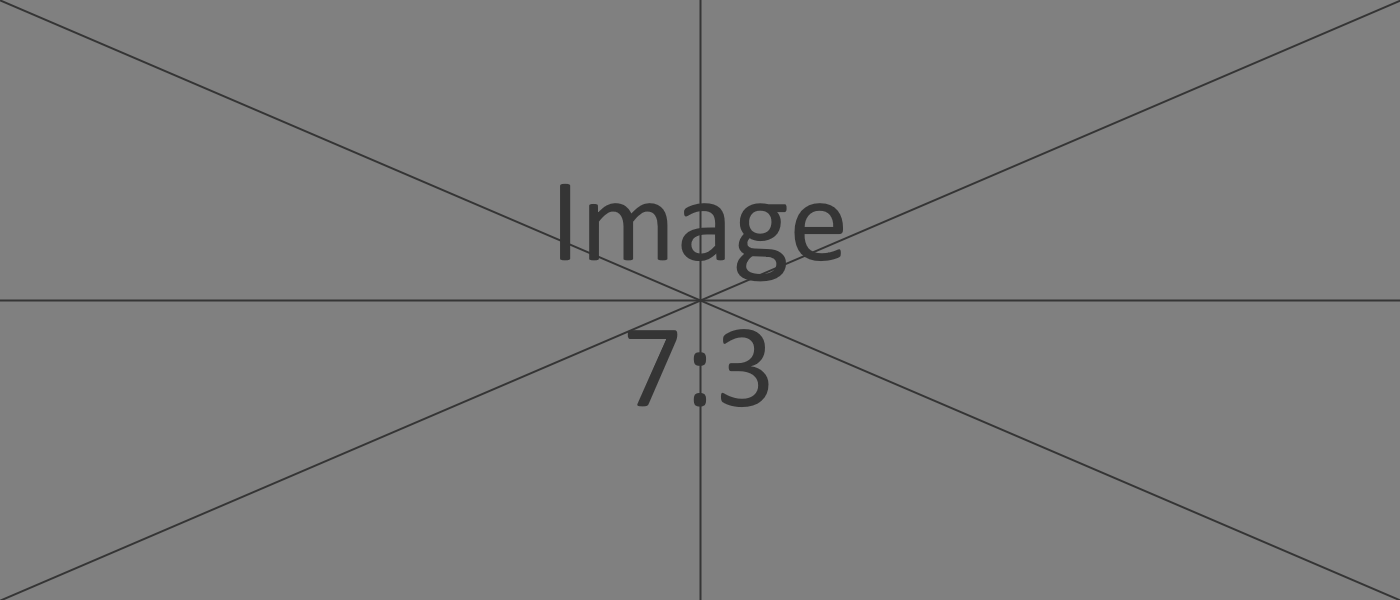
\includegraphics[width=\textwidth]{testwide.png}
	\caption[Bild 0]{\small Bild 0 seitlich dargestellt.}
	\label{abb:bild0}
\end{sidewaysfigure}
\end{lstlisting}
\begin{sidewaysfigure}
	\centering
	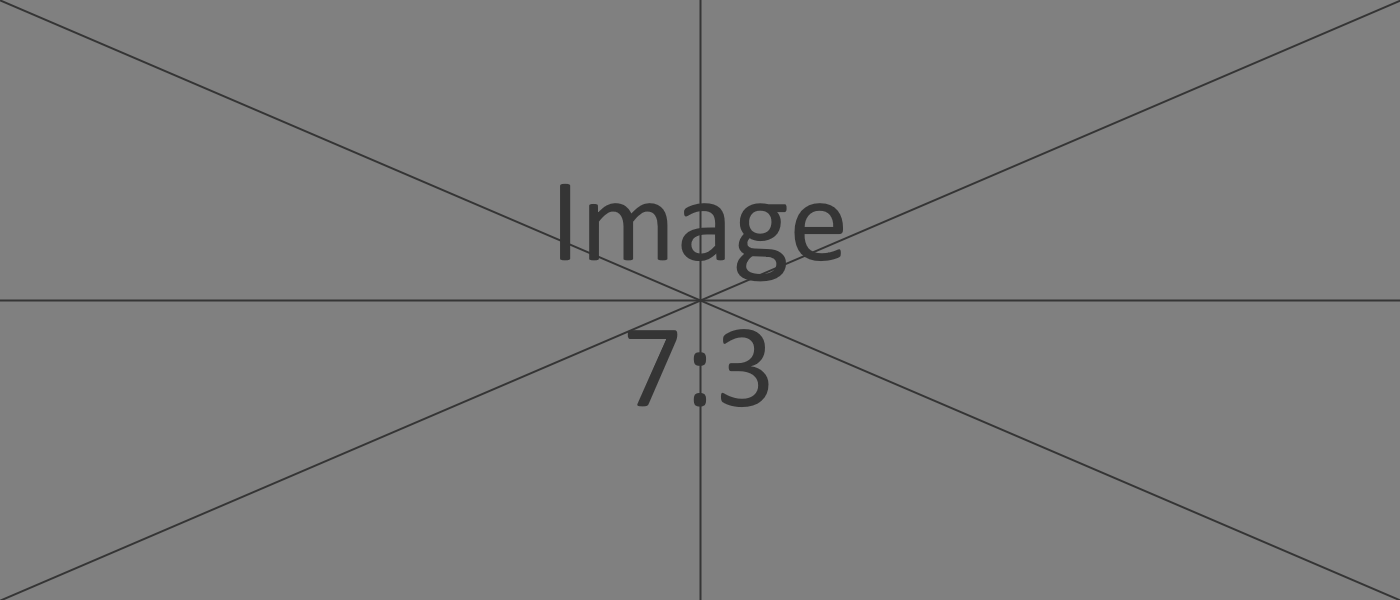
\includegraphics[width=\textwidth]{testwide.png}
	\caption[Bild 0]{\small Bild 0 seitlich dargestellt.}
	\label{abb:bild0}
\end{sidewaysfigure}

\subsection{subfigure}
\label{sec:subfigure}
Mit dem \verb|subcaption|-Paket wird die \verb|subfigure|-Umgebung definiert mit der sich Grafiken mit zugehöriger Bildunterschrift in Container packen lassen, die dann in der \verb|figure|-Umgebung eingebunden werden können.

Da es sehr viele Anordnungsmöglichkeiten gibt, wird hier nur auf einige nützliche Zusatzbefehle eingegangen gefolgt von einem großen Beispiel (siehe \autoref{fig:subfigbsp}), welches das Vorgehen veranschaulichen soll.

\begin{table}[h]
	\centering
	\caption{Nützliche Befehle für subfigure.}
	\label{tab:subfigcommands}
	\begin{tabular}{@{}L{0.27\textwidth}L{0.63\textwidth}@{}}
		\rowcolor[HTML]{000000} 
		{\color[HTML]{FFFFFF} \textbf{Befehl}} & {\color[HTML]{FFFFFF} \textbf{Beschreibung}}\\
		
		\rowcolor[HTML]{FFFFFF} 
		\verb|\hfill| & Damit wird der horizontale Platz, der übrig bleibt, frei gelassen. Das erstellt einen Abstand und macht das linke Bild links und das rechte rechtsbündig. Bei noch mehr Bildern wird der Restabstand gleichmäßig aufgeteilt.\\
		
		\rowcolor[HTML]{FFFFFF} 
		\verb|\vskip\baselineskip| & Beginn einer neuen Bildzeile.
	\end{tabular}
\end{table}

Zu beachten ist hier die Einstellung der Bildbreite von \verb|subfigure|. Eine Zeile an Bildern sollte maximal zu \SI{100}{\percent} \verb|\textwidth| aufaddiert werden können. Es ist aber meist schöner etwas mehr Platz zu lassen.

Des Weiteren sieht so eine Anordnung sehr viel besser aus, wenn die Bilder in der selben Zeile gleich groß sind. Man kann eine leichte Abweichung mit einem weißen Bildhintergrund kaschieren.

\clearpage
\begin{lstlisting}[style=latex]
\begin{figure*}[p]
	\centering
	\begin{subfigure}[b]{0.475\textwidth} \centering
		
\includegraphics[width=\textwidth]{test.png}
		\caption[Bild 1]{\small Bild 1}
		\label{abb:bild1}
	\end{subfigure}
	\hfill
	\begin{subfigure}[b]{0.475\textwidth}  \centering 
		
\includegraphics[width=\textwidth]{test.png}
		\caption[Bild 2]{\small Bild 2}    
		\label{abb:bild2}
	\end{subfigure}
	\vskip\baselineskip
	\begin{subfigure}[b]{0.475\textwidth} \centering
		
\includegraphics[width=\textwidth]{test.png}
		\caption[Bild 3]{\small Bild 3}
		\label{abb:bild3}
	\end{subfigure}
	\hfill
	\begin{subfigure}[b]{0.475\textwidth} \centering 
		
\includegraphics[width=\textwidth]{test.png}
		\caption[Bild 4]{\small Bild 4}    
		\label{abb:bild4}
	\end{subfigure}
	\vskip\baselineskip
	\begin{subfigure}[b]{\textwidth} \centering
		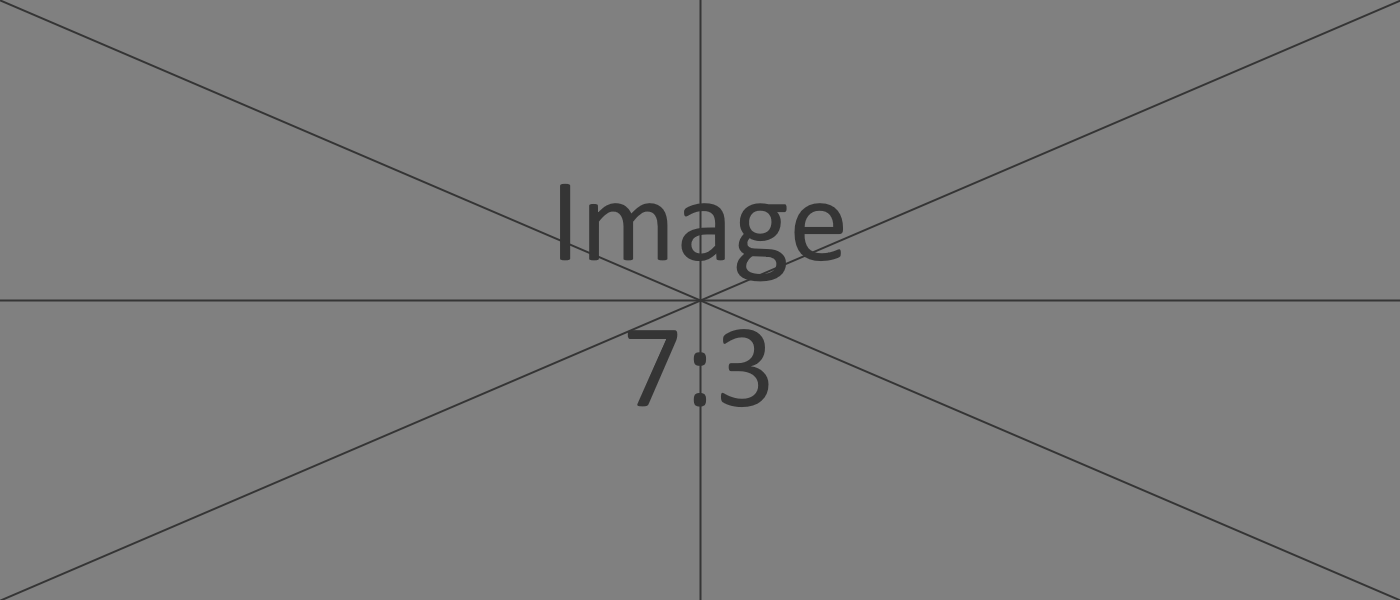
\includegraphics[width=\textwidth]{testwide.png}
		\caption[Bild 5]{\small Bild 5}
		\label{abb:bild5}
	\end{subfigure}
	\caption[Bilder Matrix]{\small Bilder Matrix} 
	\label{fig:subfigbsp}
\end{figure*}
\end{lstlisting}

\begin{figure*}[p]
	\centering
	\begin{subfigure}[b]{0.475\textwidth}
		\centering
		
\includegraphics[width=\textwidth]{test.png}
		\caption[Bild 1]{\small Bild 1}
		\label{abb:bild1}
	\end{subfigure}
	\hfill
	\begin{subfigure}[b]{0.475\textwidth}  
		\centering 
		
\includegraphics[width=\textwidth]{test.png}
		\caption[Bild 2]{\small Bild 2}    
		\label{abb:bild2}
	\end{subfigure}
	\vskip\baselineskip
	\begin{subfigure}[b]{0.475\textwidth}
		\centering
		
\includegraphics[width=\textwidth]{test.png}
		\caption[Bild 3]{\small Bild 3}
		\label{abb:bild3}
	\end{subfigure}
	\hfill
	\begin{subfigure}[b]{0.475\textwidth}  
		\centering 
		
\includegraphics[width=\textwidth]{test.png}
		\caption[Bild 4]{\small Bild 4}    
		\label{abb:bild4}
	\end{subfigure}
	\vskip\baselineskip
	\begin{subfigure}[b]{\textwidth}
		\centering
		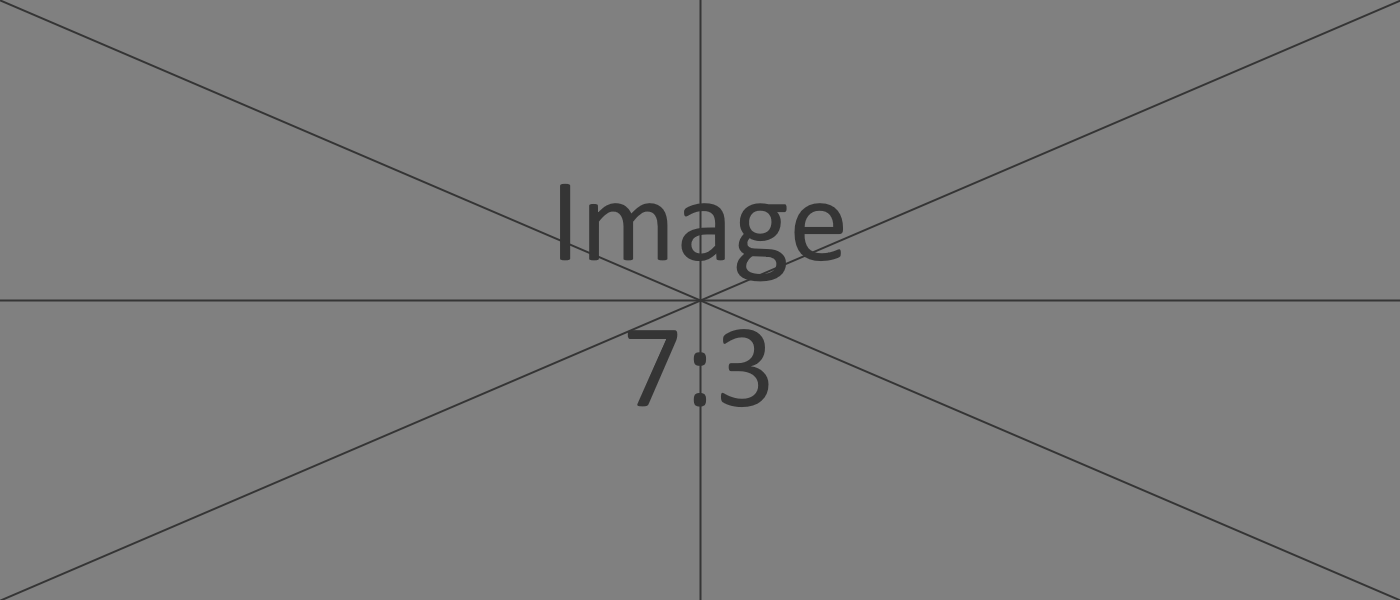
\includegraphics[width=\textwidth]{testwide.png}
		\caption[Bild 5]{\small Bild 5}
		\label{abb:bild5}
	\end{subfigure}
	\caption[Bilder Matrix]{\small Bilder Matrix} 
	\label{fig:subfigbsp}
\end{figure*}

\subsection{Extra}
Das Beispiel kommt von David Carlisle\cite{DavidCarlisle}.
Möchte man zwei Bilder unterschiedlicher Größe nebeneinander darstellen und dabei sicher gehen, dass keines der beiden Bilder verzerrt wird und am Ende beide gleich hoch sind und nur eine maximale Breite haben, kann einem dieses Beispiel helfen:

\begin{lstlisting}[style=latex]
\begin{figure}[h]
	% preliminary
	\sbox\twosubbox{
		\resizebox{\dimexpr.80\textwidth-1em}{!}{
			
\includegraphics[height=200pt]{test.png}
			
\includegraphics[height=200pt]{test2.png}
		}
	}
	\setlength{\twosubht}{\ht\twosubbox}
	
	% typeset
	\centering
	\subcaptionbox{$4:3$-Bild, Größe=800x600\label{abb:testimage_1}}{
		
\includegraphics[height=\twosubht]{test.png}%
	}\quad
	\subcaptionbox{$1:1$-Bild, Größe=400x400\label{abb:testimage_2}}{
		
\includegraphics[height=\twosubht]{test2.png}
	}
	\caption[Beide Abbildungen]{\small Beide Abbildungen}
	\label{fig:both_testimages}	
\end{figure}
\end{lstlisting}

In Zeile 4 kann der Faktor vor \verb|\textwidth| angepasst werden und damit die gesamt Breite beider Bilder. Die Höhe wird dann automatisch errechnet und angepasst. Der Wert \verb|height=200pt| in Zeile 5 und 6 kann angepasst werden, beeinflusst aber höchstens die Auflösung mit der die Bilder eingebunden werden. Es ist wichtig, dass dieser Wert bei beiden gleich ist!

\begin{figure}[H]
	% preliminary
	\sbox\twosubbox{
		\resizebox{\dimexpr.80\textwidth-1em}{!}{
			
\includegraphics[height=200pt]{test.png}
			
\includegraphics[height=200pt]{test2.png}
		}
	}
	\setlength{\twosubht}{\ht\twosubbox}
	
	% typeset
	\centering
	\subcaptionbox{$4:3$-Bild, Größe=800x600\label{abb:testimage_1}}{
		
\includegraphics[height=\twosubht]{test.png}%
	}\quad
	\subcaptionbox{$1:1$-Bild, Größe=400x400\label{abb:testimage_2}}{
		
\includegraphics[height=\twosubht]{test2.png}
	}
	
	\caption[Beide Abbildungen]{\small Beide Abbildungen}
	\label{fig:both_testimages}	
\end{figure}

\section{Tabellen}
Tabellen werden in \LaTeX{} ähnlich wie Bilder gehandhabt. Man definiert die \verb|table|-Um\-ge\-bung als äußeren Wrapper für die Tabelle, ähnlich wie die \verb|figure|-Um\-ge\-bung bei Abbildungen.
In dieser Umgebung erstellt man die \verb|tabular|-Umgebung, in der man nun den Inhalt der einzelnen Zeilen und Spalten definiert.
\begin{lstlisting}[style=latex]
\begin{table}[htb]
	\centering
	\caption{Tabellen Beispiel}
	\label{tab:beispieltabelle}
	\begin{tabular}{rrr} % 3 spalten rechtsbündig
		\toprule
		Zeit & $\sin$-Funktion & $\cos$-Funktion\\
		\midrule
		$0.0000$ & $0.00000$ & $1.0000$ \\
		$1.0000$ & $0.84147$ & $0.54030$ \\
		$2.0000$ & $0.90930$ & $-0.41615$ \\
		$3.0000$ & $0.14112$ & $-0.98999$ \\
		$4.0000$ & $-0.75680$ & $-0.65364$ \\
		$5.0000$ & $-0.95892$ & $0.28366$ \\
		$6.0000$ & $-0.27942$ & $0.96017$ \\ % usw.
		\bottomrule
	\end{tabular}
\end{table}
\end{lstlisting}

\subsection{table}
Die \verb|table|-Umgebung ist so ziemlich das gleiche, wie die \verb|figure|-Umgebung für Abbildungen. Es kann wieder mit den Optionen (siehe \autoref{tab:figureoptions}) die Position bestimmt werden. Einzig zu beachten ist, dass bei Tabellen die \verb|caption| oberhalb der Tabelle steht.

\subsection{tabular}
Mit \verb|tabular| wird die eigentlich Tabelle erzeugt. Der zweite Parameter konfiguriert dabei die einzelnen Spalten und die Trennstriche dazwischen. 
\begin{table}[ht]
	\centering
	\caption{Spaltenoptionen in einem anderen Design}
	\label{tab:beispieltabelle}
	\begin{tabular}{|l|l|}
		\hline
		\textbf{Option} & \textbf{Beschreibung}\\
		\hline
		\verb|l| & Spalte mit linksbündigem Text\\
		\hline
		\verb|c| & Spalte mit mittigem Text\\
		\hline
		\verb|r| & Spalte mit rechtsbündigem Text\\
		\hline
		\verb=|= & Trennstrich zwischen der linken und rechten Spalte\\
		\hline
		\verb|L{space}| & \verb|space|-Breite Spalte mit linksbündigem Text\\
		\hline
		\verb|C{space}| & \verb|space|-Breite Spalte mit mittigem Text\\
		\hline
		\verb|R{space}| & \verb|space|-Breite Spalte mit rechtsbündigem Text\\
		\hline
	\end{tabular}
\end{table}

Der eigentliche Inhalt erfolgt dann Zeilenweise, die jeweils, mit Ausnahme der letzten, mit einem \verb|\\| beendet wird. (Außer ihr fügt am Ende noch eine Endlinie hinzu, dann wird auch die letzte Zeile mit einem \verb|\\| beendet.) 
Die einzelnen Spalten werden dabei mit dem \verb|&| Zeichen getrennt. Es müssen in jeder Zeile alle Spalten angegeben werden, auch wenn diese leer bleiben. 
\begin{figure}[h] 
	\begin{minipage}[t]{0.47\textwidth} 
		\begin{lstlisting}[style=latex]
\begin{tabular}{|l|c|r|}
	\hline
	1 & 2 & 3\\
	\hline
	4 & 5 & 6\\
	\hline
	7 & 8 & 9\\
	\hline
	& 0 & \\
	\hline
\end{tabular}
\end{lstlisting}
	\end{minipage} 
	% 
	\begin{minipage}[t]{0.47\textwidth} 
		\centering
		\caption*{Beispiel 1}
		\begin{tabular}{|l|c|r|}
			\hline
			1 & 2 & 3\\
			\hline
			4 & 5 & 6\\
			\hline
			7 & 8 & 9\\
			\hline
			& 0 & \\
			\hline
		\end{tabular}
	\end{minipage} 
\end{figure} 

Mit \verb|\multirow| und \verb|\multicolumn| können auch Zellen verbunden werden.
\begin{figure}[h] 
	\begin{minipage}[t]{0.47\textwidth} 
\begin{lstlisting}[style=latex]
\begin{tabular}{|c|c|c|}\hline
	1 & 2 & 3\\
	\hline
	& \multicolumn{2}{c|}{5}\\
	\cline{2-3}
	\multirow{-2}{*}{4} & 6 & 7\\
	\hline
\end{tabular}
\end{lstlisting}
	\end{minipage} 
	% 
	\begin{minipage}[t]{0.47\textwidth} 
		\centering
		\caption*{Beispiel 2}
		\begin{tabular}{|c|c|c|}\hline
			1 & 2 & 3\\\hline
			& \multicolumn{2}{c|}{5}\\\cline{2-3}
			\multirow{-2}{*}{4} & 6 & 7\\\hline
		\end{tabular}
	\end{minipage} 
\end{figure} 

Für eine genaue Erklärung der Funktionsweise schauen Sie in die Dokumentation zu\\\verb|multirow| und \verb|multicolumn|.

\subsection{Beispieltabelle}
\begin{lstlisting}[style=latex]
\begin{table}[h]
	\centering
	\caption{Beispieltabelle 1}
	\label{tab:bsp1}
	\begin{tabular}{@{}C{0.15\textwidth}L{0.75\textwidth}@{}}
		\rowcolor[HTML]{000000} 
		{\color[HTML]{FFFFFF} \textbf{Nummer}} & {\color[HTML]{FFFFFF} \textbf{Beschreibung}}\\
		\rowcolor[HTML]{FFFFFF} 
		\num{1} & Beschreibung 1\\
		\rowcolor[HTML]{C0C0C0} 
		\num{2} & Beschreibung 2\\
		\rowcolor[HTML]{FFFFFF} 
		\num{3} & Beschreibung 3\\
		\rowcolor[HTML]{C0C0C0} 
		\num{4} & Beschreibung 4
	\end{tabular}
\end{table}
\end{lstlisting}
\begin{table}[h]
	\centering
	\caption{Beispieltabelle 1}
	\label{tab:bsp1}
	\begin{tabular}{@{}C{0.15\textwidth}L{0.75\textwidth}@{}}
		\rowcolor[HTML]{000000} 
		{\color[HTML]{FFFFFF} \textbf{Nummer}} & {\color[HTML]{FFFFFF} \textbf{Beschreibung}}\\
		
		\rowcolor[HTML]{FFFFFF} 
		\num{1} & Beschreibung 1\\
		
		\rowcolor[HTML]{C0C0C0} 
		\num{2} & Beschreibung 2\\
		
		\rowcolor[HTML]{FFFFFF} 
		\num{3} & Beschreibung 3\\
		
		\rowcolor[HTML]{C0C0C0} 
		\num{4} & Beschreibung 4
	\end{tabular}
\end{table}

\subsection{Tabellen Generator}
Wer ein anderes Design für seine Tabellen haben möchte, kann sich ein eigenes Design mithilfe der Webseite \url{https://www.tablesgenerator.com/#} erstellen. Es sei aber Angemerkt, dass darauf geachtet werden sollte, dass die Arbeit in sich konsistent und nicht zu überladen ist, also nicht jede Tabelle ein anderes Design mit einer ausgiebigen Farb\-über\-flut\-ung hat.

\section{Quelltext}
Quellcode kann mit dem \verb|lstlisting|-Paket eingebunden werden. Für \verb|C++|, \verb|Matlab|, \verb|VHDL| und \verb|Latex|-Code wird der Quelltext auch automatisch entsprechend dargestellt. 

Quelltext kann auf zwei verschiedene arten eingebunden werden. Zum einen kann mit dem \verb|\lstinputlisting|-Befehl direkt eine Quelldatei angegeben werden, zum anderen ist es auch möglich den Quelltext direkt in der \verb|lstlisting|-Umgebung zu schreiben (Siehe \autoref{lst:bsp}).
\vspace{5mm}
\begin{lstlisting}[style=latex]
\lstinputlisting[style=matlab,caption={Beispiel}]{Quelltext/Beispiel.m}
\end{lstlisting}
\lstinputlisting[style=matlab,caption={Beispiel}]{Quelltext/Beispiel.m}

\begin{lstlisting}[style=latex,mathescape=true]
\$$begin{lstlisting}[style=cpp,caption={Beispiel C++},label=lst:bsp]
	..Quelltext..
\$$end{lstlisting}
\end{lstlisting}
\begin{lstlisting}[style=cpp,caption={Beispiel C++},label=lst:bsp]
#include <iostream>
int main{
	std::cout << "Hallo Welt!" << std::endl;
	return 0;
}
\end{lstlisting}

Hier eine liste aller Styles die bereits in \verb|Vorspann_Dipl.tex| definiert wurden.
\begin{table}[h]
	\centering
	\caption{Styles für die lstlisting-Umgebung}
	\label{tab:lstlistingstyle}
	\begin{tabular}{@{}L{0.2\textwidth}L{0.2\textwidth}@{}}
		\rowcolor[HTML]{000000} 
		{\color[HTML]{FFFFFF} \textbf{Kürzel}} & {\color[HTML]{FFFFFF} \textbf{Sprache}}\\
		
		\rowcolor[HTML]{FFFFFF} 
		\verb|Matlab| & Matlab\\
		
		\rowcolor[HTML]{C0C0C0} 
		\verb|cpp| & C++\\
		
		\rowcolor[HTML]{FFFFFF} 
		\verb|vhdl| & VHDL\\
		
		\rowcolor[HTML]{C0C0C0} 
		\verb|latex| & Latex\\
	\end{tabular}
\end{table}

\section{Extras}
\subsection{Paket Dokumentationen}
Um die Dokumentation eines installierten Pakets anzusehen ist der \verb|texdoc|-Befehl hilfreich.
\begin{lstlisting}
	texdoc paketname
\end{lstlisting}
Bei Windows einfach in der Eingabeaufforderung oder im Ausführen Dialog eingeben und es sollte sich die jeweilige Dokumentation öffnen. Bei Linux und Mac sollte das im Terminal genauso funktionieren.

\subsection{Kein Perl}\label{sec:noperl}
Wenn Perl keine Option ist, kann alternativ versucht werden das \verb|Makeindex|-Skript zu benutzen. Dazu geht man mit der Kommandozeile in den Ordner mit den \textit{.tex}-Dateien und versucht es mit:
\begin{lstlisting}
	makeindex.exe -s %.ist -t %.alg -o %.acr %.acn
	makeindex.exe -s %.ist -o %.sym %.sbl
\end{lstlisting}
\textbf{Achtung:} \verb|%| steht für den Namen der Hauptdatei!
Sollte das nicht funktionieren bemühen Sie die Suchmaschine ihrer Wahl und schauen Sie sich die Dokumentation des \verb|glossaries|-Pakets an.
